\documentclass[11pt,a4paper]{article}
\usepackage[margin=2.5cm]{geometry}
\usepackage{booktabs}
\usepackage{graphicx}
\usepackage{xcolor}
\usepackage{hyperref}
\usepackage{enumitem}
\usepackage{titlesec}
\usepackage{fancyhdr}
\usepackage{microtype}
\usepackage{parskip}
\usepackage{fontspec}
\usepackage{polyglossia}
\usepackage{amsmath}
\usepackage{amssymb}

\setmainlanguage{english}
\setotherlanguage{hebrew}
\newfontfamily\hebrewfont{DejaVu Sans}[Script=Hebrew]

\hypersetup{colorlinks=true, linkcolor=blue, urlcolor=blue}

\pagestyle{fancy}
\fancyhf{}
\rhead{Knesset Protocol Journal Project}
\lhead{Step 4 --- Hybrid TF-IDF + Dense}
\rfoot{Page \thepage}
\lfoot{Tomer Morad, Or Israeli, Yoel Marko --- June 2026}

\titleformat{\section}{\large\bfseries}{\thesection.}{0.6em}{}[\titlerule]
\titleformat{\subsection}{\normalsize\bfseries}{\thesubsection}{0.6em}{}

\begin{document}

\begin{center}
  {\LARGE \textbf{Hybrid TF-IDF + ABTT Dense Score Fusion}}\\[0.3em]
  {\large Step 4 --- Combining lexical precision with semantic recall}\\[0.6em]
  {\normalsize Tomer Morad \quad Or Israeli \quad Yoel Marko}\\
  {\normalsize June 2026}
\end{center}

\vspace{0.5em}

% ----------------------------------------------------------------------
\section{Objective}

Steps 2--3 established two complementary similarity signals:
\begin{itemize}[noitemsep]
  \item \textbf{TF-IDF} captures \emph{lexical} discriminators: bill identifiers
        (\texthebrew{מ/1610}, \texthebrew{פ/NNNN}), law names, and domain-specific terminology.
        High precision on exact-match topics, brittle to paraphrase.
  \item \textbf{ABTT-corrected dense} (AlephBERT $k=2$, \texttt{e5} $k=1$) captures
        distributional/semantic similarity after projecting out the register bias.
        Robust to paraphrase and surface variation, but less sharp on entity-centric topics.
\end{itemize}

This step tests whether combining them via \textbf{score fusion} yields a strictly better
similarity score for the subject-linking task.

% ----------------------------------------------------------------------
\section{Method}

Given precomputed L2-normalized similarity matrices $S_\text{tfidf}$ and $S_\text{dense}$
(both $105 \times 105$ on the recurring subset), the hybrid score is:
\[
  S_\text{hybrid}(\alpha) \;=\; \alpha \cdot S_\text{tfidf} \;+\; (1-\alpha) \cdot S_\text{dense},
  \qquad \alpha \in \{0.0,\, 0.1,\, \ldots,\, 1.0\}.
\]
$\alpha = 0$ is pure dense; $\alpha = 1$ is pure TF-IDF.  Both endpoint cases
reproduce the Step 2/3 baselines.

\textbf{Clustering uses $S_\text{hybrid}$ directly:}
\begin{itemize}[noitemsep]
  \item \emph{Agglomerative}: precomputed distance $= 1 - S_\text{hybrid}$, average linkage,
        $K=28$.
  \item \emph{Spectral}: precomputed affinity $= \max(S_\text{hybrid}, 0)$, $K=28$.
\end{itemize}

Four ABTT variants are tested: \texttt{alephbert\_k2}, \texttt{e5\_k3} (best KMeans in Step 3),
\texttt{e5\_k1} (best agglomerative/AUC in Step 3), and \texttt{mpnet\_k10}.

% ----------------------------------------------------------------------
\section{Results}

\subsection{Summary table}

\begin{center}
\begin{tabular}{lcccc}
\toprule
\textbf{Configuration} & \textbf{Best $\alpha$} & \textbf{ARI$_\text{agg}$} & \textbf{ARI$_\text{spec}$} & \textbf{AUC} \\
\midrule
\textbf{TF-IDF only} & --- & 0.249 & 0.335 & 0.741 \\
\midrule
\texttt{alephbert\_k2}, pure ($\alpha=0$) & --- & 0.513 & 0.377 & 0.887 \\
\textbf{\texttt{alephbert\_k2}}, $\alpha=0.6$ & \textbf{0.6} & \textbf{0.569} & \textbf{0.519} & 0.879 \\
\midrule
\texttt{e5\_k1}, pure ($\alpha=0$) & --- & 0.540 & 0.417 & \textbf{0.899} \\
\texttt{e5\_k1}, $\alpha=0.4$ & 0.4 & 0.540 & 0.400 & 0.895 \\
\midrule
\texttt{e5\_k3}, $\alpha=0.8$ & 0.8 & 0.503 & 0.441 & 0.826 \\
\texttt{mpnet\_k10}, $\alpha=0.9$ & 0.9 & 0.351 & 0.378 & 0.755 \\
\bottomrule
\end{tabular}
\end{center}

\noindent\textbf{Global best:} \texttt{alephbert\_k2} at $\alpha=0.6$, ARI$_\text{agg}=0.569$
--- a \textbf{2.3$\times$} improvement over TF-IDF alone.

\begin{center}
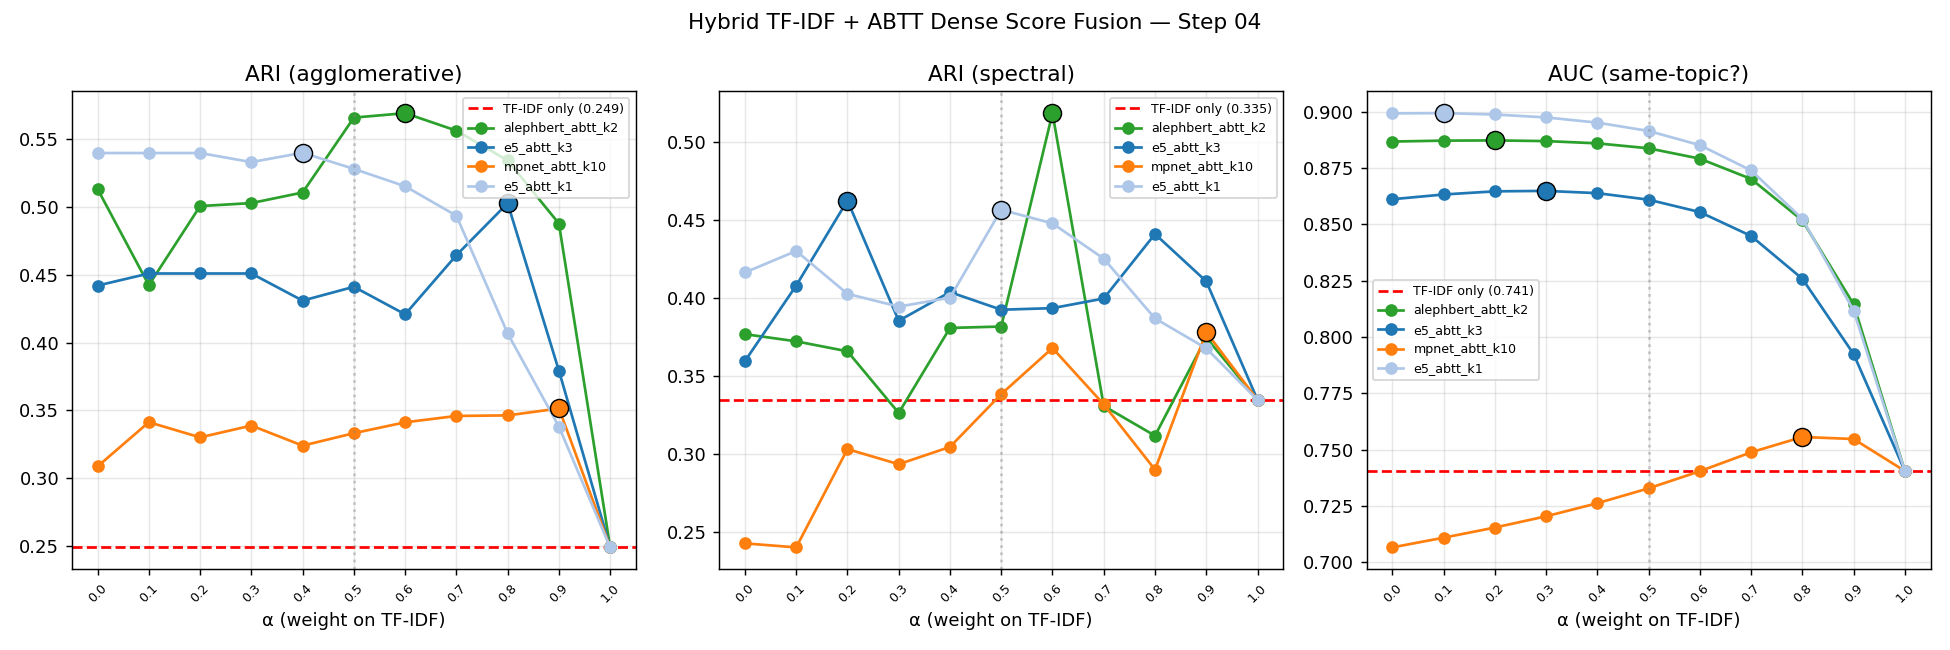
\includegraphics[width=\textwidth]{../outputs/hybrid_curves.png}
\end{center}
\noindent KMeans ARI, Agglomerative ARI, and AUC as a function of $\alpha$ for each ABTT
variant.  Red dashed line = TF-IDF only.  Filled circles mark the best $\alpha$ per model.
Left end ($\alpha=0$) = pure dense; right end ($\alpha=1$) = pure TF-IDF.

\subsection{Model-specific behaviour}

\paragraph{AlephBERT $k=2$ (best clustering).}
The hybrid strictly dominates both components: $\alpha=0.6$ (slightly TF-IDF-weighted) gives
ARI$_\text{agg}=0.569$ vs.\ 0.513 for pure dense.  The two signals carry complementary
information: AlephBERT captures committee-specific paraphrase; TF-IDF captures bill numbers
that identify the exact legislative matter.

\paragraph{\texttt{e5} $k=1$ (best AUC).}
The $\alpha$ curve is essentially flat from 0 to 0.4 (ARI$_\text{agg}\approx0.540$),
suggesting that \texttt{e5} $k=1$ has already internalized the lexical discriminators to
the extent that TF-IDF adds no additional information.  AUC = 0.899 throughout.
\textbf{This model is the natural choice for the Task-2 similarity baseline.}

\paragraph{mpnet.}
Performance improves marginally with TF-IDF mixing but never approaches AlephBERT or e5.
mpnet is excluded from further steps.

\subsection{AUC is maximized by pure dense}

Adding TF-IDF degrades AUC monotonically (TF-IDF's own similarity gap is only 0.069 vs.\
dense $\approx$0.34).  For \emph{ranking} purposes (retrieval pre-filter for the LLM verifier),
pure dense with \texttt{e5} $k=1$ or \texttt{alephbert} $k=2$ is optimal.

% ----------------------------------------------------------------------
\section{Takeaways}

\begin{itemize}[noitemsep]
  \item \textbf{Score fusion helps AlephBERT but not e5.}  The difference reflects the
        models' handling of entity-centric signal: AlephBERT, trained on raw Hebrew text,
        benefits from the explicit lexical overlay; e5, contrastively trained, absorbs
        that signal on its own.
  \item \textbf{Two operating points for downstream use:}
        \texttt{alephbert\_k2} at $\alpha=0.6$ for clustering (ARI$_\text{agg}=0.569$);
        \texttt{e5\_k1} pure dense for ranking/AUC (0.899).
  \item \textbf{Score fusion is a zero-cost improvement}: no retraining, no new data,
        linear combination of precomputed similarity matrices.
\end{itemize}

% ----------------------------------------------------------------------
\section{Future Directions}

\begin{enumerate}[leftmargin=1.4em]
  \item \textbf{Similarity threshold baseline (Task 2a).}  Use the best representations
        to set an operating point for the online LINK/NEW decision and characterize the
        precision--recall trade-off under the anti-duplication constraint.  (Step 5.)
  \item \textbf{LLM verifier (Task 2b).}  Use \texttt{e5\_k1} as a retrieval pre-filter
        (top-$K$ candidates) and a prompted LLM as verifier.
  \item \textbf{Fine-grained $\alpha$ sweep} around 0.5--0.7 for AlephBERT (0.05 steps)
        to pinpoint the optimal mixing weight.
  \item \textbf{Entity-weighted TF-IDF.}  Give extra weight to bill-ID tokens
        (\texthebrew{מ/NNNN}) and named entities identified by an NER model to sharpen
        the lexical component.
\end{enumerate}

\vspace{1.5em}
\hrule
\vspace{0.4em}
{\small
\textbf{Artifacts (this step):}
\texttt{outputs/hybrid\_results.json},
\texttt{outputs/hybrid\_curves.png},
\texttt{outputs/best\_sim\_matrix.npy} (\texttt{alephbert\_k2}, $\alpha=0.6$).\\
\textbf{Code:} \texttt{code/hybrid\_eval.py}.
}

\end{document}
